\chapter{Влияние шероховатой поверхности на кинетические эффекты в низкоразмерных системах} \label{chapt3}

\section{ Подвижность носителей в размерно-квантованных системах с учетом рассеяния на поверхности и фононах}

Квантовые системы с пониженной размерностью (квантовые ямы (КЯ), сверхрешетки, квантовые проволоки (КП)) благодаря их уникальным свойствам, связанным с возникновением размерного квантования, продолжают привлекать внимание теоретиков и экспериментаторов. При этом кинетические явления в размерно-квантованных системах принципиальным образом отличаются от объемных материалов. Так, например, в объемных материалах сопротивление растет с увеличением температуры $T$, а в КП малого диаметра $d$ ($d \sim 70 \AA$) убывает, оставаясь практически постоянным в области низких $T$ \cite{Lin2000,Lin2003,Heremans1998,Zhang2000,Heremans2000}. Для КЯ GaAs/AlAs температурная зависимость подвижности $\mu (T)$ может носить не монотонный характер: в области низких температур (T$>$10K) $\mu (T)$ увеличивается с ростом T, а при $T>100K$ начинает уменьшаться \cite{Lin2000,Sakaki1987}. Следовательно, размеры квантовых систем принципиальным образом могут влиять на величину и температурную зависимость электропроводности.

В данной главе делается попытка объяснить особенности температурной зависимости электропроводности, экспериментально наблюдаемые в нелегированных наноструктурах, учитывая процессы рассеяния носителей на шероховатой поверхности и на фононах. Именно из сравнения теоретических результатов с экспериментальными данными по температурной зависимости электропроводности можно провести оценки параметров флуктуирующей поверхности. Учет двух механизмов рассеяния позволил сформулировать условия на ширину размерно-ограниченной системы и температуру, когда рассеяние электронов на фононах преобладает над рассеянием носителей на шероховатой поверхности.

Расчет электропроводности проводится согласно формуле Кубо \cite{Kubo1957a} для статической электропроводности, которая в представлении вторичного квантования имеет вид \footnote{ Полученное выражение для электропроводности справедливо для любых квантовых систем в произвольном магнитном поле. Единственное ограничение -- это малость электрического поля, т.е. область применимости закона Ома.}:
\begin{equation} \label{eq:31_10}
\sigma _{ij} =\frac{\beta_0 e^2 }{2 V m^2 } \sum _{\alpha,\beta, \alpha_1,\beta_1} \hat{p}_{\alpha \beta }^{(i)} \hat{p}_{\alpha_1 \beta }^{(j)} \int\limits_{-\infty }^{\infty} {dt\left\langle a_{\alpha }^+ (t) a_{\beta }(t) a_{\alpha_1 }^+ a_{\beta_1 } \right\rangle}
\end{equation} 
$\hat{p}_{\alpha \beta }^{(i)} $~---~матричный элемент оператора импульса на сглаженных волновых функциях зонного электрона, $\beta_0 = 1/k_0 T$, $\alpha $~---~квантовые числа, описывающие состояние заряженной частицы с эффективной массой m, $V$~---~объем основной области системы,
\[
a_{\alpha }^+ (t)= \exp\left(\frac{it\hat{H}}{\hbar } \right)a_{\alpha }^+ \exp\left(-\frac{it\hat{H}}{\hbar } \right),
\] 
$\left\langle \cdot \cdot \cdot \right\rangle $~---~описывает усреднение по системе равновесных электронов и по реализации случайного процесса.

Гамильтониан для электрона, взаимодействующего с шероховатой поверхностью размерно-ограниченной системы в представлении вторичного квантования записывается в виде:
\begin{equation} \label{eq:31_20}
\hat{H}=\sum _{\alpha }\varepsilon _{\alpha } a_{\alpha }^{+} a_{\alpha } +\sum _{\alpha ,\beta }{\left\langle \alpha  \right|} \hat{V}{\left| \beta  \right\rangle} a_{\alpha }^{+} a_{\beta }, 
\end{equation}
$\hat{V}$~---~оператор взаимодействия носителя с энергией $\varepsilon _{\alpha } $ с поверхностью системы, ${\left| \alpha  \right\rangle} $~---~волновая функция зонного электрона.

С гамильтонианом \eqref{eq:31_20} расчет временной зависимости операторов
рождения $a_\alpha ^ + (t)$ и уничтожения $a_\alpha (t)$ можно
провести точно по аналогии \cite{Khamidullin2002}. В результате
\begin{equation}
\begin{array}{c}\label{eq:31_23}
\displaystyle a_\alpha ^ + (t) = \exp\left(
{\frac{it\varepsilon _\alpha }{\hbar }} \right)\sum\limits_\beta
{a_\beta ^ + \left\langle \beta \right|} \exp\left[
{\frac{it}{\hbar }\left( {\hat {H}_0 + V} \right)}
\right]\exp\left( { - \frac{it}{\hbar }\hat {H}_0 }
\right)\left| \alpha \right\rangle ,\\
\displaystyle a_\alpha (t) = \exp\left( { - \frac{it\varepsilon
		_\alpha }{\hbar }} \right)\sum\limits_\beta {\left\langle \alpha
	\right|} \exp\left( {\frac{it}{\hbar }\hat {H}_0 }
\right)\exp\left[ { - \frac{it}{\hbar }\left( {\hat {H}_0 + V}
	\right)} \right]\left| \beta \right\rangle a_\beta .
\end{array},
\end{equation}
здесь обозначено: $\hat {H}_0 $ -- гамильтониан для свободных
носителей в координатном представлении $\left( \hat {H}_0 \left| \alpha
\right\rangle = \varepsilon _\alpha \left| \alpha \right\rangle
\right) $.

Если подставить \eqref{eq:31_23}  в \eqref{eq:31_10}, выражение для
электропроводности принимает следующий вид:
\begin{multline}
\sigma_{ij}=\frac{\beta_0e^2}{2Vm^2}\sum\limits_{\alpha	,\beta ,\alpha _1 ,\beta _1, \atop \gamma ,\gamma _1 } 
\hat{p}_{\alpha \beta}^{(i)} \hat {p}_{\alpha _1 \beta_1}^{(j)}
\int\limits_{- \infty }^\infty
{dt \left\{ \left\langle \gamma \left|\exp\left[\frac{it}{\hbar}\left(\hat{H}_0 + V\right)\right]\right|\alpha\right\rangle\right.}\times\\
\times\displaystyle\left.\left\langle \beta
\left|\exp\left[-\frac{it}{\hbar}\left(\hat {H}_0 +
V\right)\right]\right|\gamma_1\right\rangle\right\}_V \left\langle
{a_\alpha ^ + a_{\gamma _1 } a_{\alpha _1 }^ + a_{\beta _1 } }
\right\rangle _0,
\end{multline}
$\left\langle
{...} \right\rangle _0 $-- усреднение с равновесной матрицей
плотности для электронов.

Согласно теореме Вика:
\begin{equation}\label{eq:31_26}
\left\langle {a_\gamma ^ + a_{\gamma _1 } a_{\alpha _1
	}^ + a_{\beta _1 } } \right\rangle _0 = n_\gamma \left( {1 -
	n_{\gamma _1 } } \right)\delta _{\gamma \beta _1 } \delta _{\gamma
	_1 \alpha _1 } + n_\gamma n_{\alpha _1 } \delta _{\gamma \gamma _1
} \delta _{\alpha _1 \beta _1 } ,
\end{equation}
$n_\alpha = \left\{ {\exp\left[ {\beta \left( {\varepsilon _\alpha - \xi } \right)} \right] + 1} \right\}^{ - 1}$~---~равновесная
функция распределения для электронов с энергией $\varepsilon{_\alpha}$, $\xi $~---~химический потенциал.

С учетом первого слагаемого \eqref{eq:31_26} диагональный тензор
электропроводности описывается соотношением:
\begin{multline}\label{eq:31_30}
\displaystyle\sigma_{ij}=\frac{\beta_0 e^2}{2Vm_e^2}
\sum\limits_{\alpha,\beta ,\beta_1 ,\alpha_1 } \hat {p}_{\alpha \beta}^{(i)} \hat{p}_{\alpha_1 \beta_1}^{(j)}
n_{\beta_1} \left( 1 - n_{\alpha_1}\right)\times\\
\times\int\limits_{- \infty }^\infty {dt \left\{ \left\langle\beta_1 \left| \exp\left[\frac{it}{\hbar}\left(\hat{H}_0 + V\right)\right]	\right|\alpha\right\rangle \right.} \displaystyle\left.\left\langle \beta\right|\exp\left[-\frac{it}{\hbar}\left(\hat{H}_0 + V\right)\right] \left|\alpha_1\right\rangle\right\}_V
\end{multline}
${\left\{\cdots \right\}}_V$~---~описывает усреднение по реализации случайного процесса $\Delta \left(x,y\right)$.

В дальнейшем проведем усреднение для матричных элементов в \eqref{eq:31_30} независимо. Такое приближение соответствует приближению «времени релаксации» \cite{Khamidullin2002} и конечные результаты для кинетических коэффициентов будут вероятно отличаться от тех, которые получаются при использовании решения классического уравнения Больцмана. 

Рассмотрим функцию
\begin{multline} \label{eq:31_40}
y_{{\beta }_1\alpha }=\exp\left(-\frac{it}{\hbar }E_{\beta_1}\right){\left\{\left\langle {\beta }_1\left|\exp\left[ {\frac{it}{\hbar }\left( {\hat {H}_0 + V} \right)} \right]\right|\alpha \right\rangle \right\}}_V=\\
={\left\{\left\langle {\beta }_1\left|T{\exp_{[-]} \left[\frac{i}{\hbar }\int^{\infty }_0{V\left(\tau \right)d \tau }\right]\ }\right|\alpha \right\rangle \right\}}_V,
\end{multline}
здесь обозначено:
\[
T{\exp_{\left[-\right]} \left[\frac{i}{\hbar }\int\limits^{\infty }_0 {V\left(\tau \right)d \tau } \right]}
	=\exp\left( {-\frac{it}{\hbar }\hat {H}_0 }\right)\exp\left[ {\frac{it}{\hbar }\left( {\hat {H}_0 + V} \right)} \right],
\] 
\[
V(\tau ) = \exp\left( {\frac{i\tau \hat {H}_0 }{\hbar }}\right)
V\exp\left( { - \frac{i\tau \hat {H}_0 }{\hbar }} \right).
\]
Усреднение по реализации случайного процесса в \eqref{eq:31_40} проведем с использованием кумулянтного усреднения \cite{Kubo1957a}. Тогда, выражение \eqref{eq:31_40} с точностью до второй кумулянты принимает следующий вид:
\[
y_{{\beta }_1\alpha }\left(t\right)=\left\langle {\beta }_1\left|{\exp \left\{-\frac{1}{{\hbar }^2}\int^t_0{d \tau \int^{\tau }_0{d {\tau }_1{\left\{V\left({\tau }_1\right)V\left(\tau \right)\right\}}_V}}\right\}\ }\right|\alpha \right\rangle
\]
Не трудно показать, что
\begin{equation} \label{eq:31_60}
{\dot{y}}_{{\beta }_1\alpha }\left(t\right)=-\frac{1}{{\hbar }^2}\int^t_0{d \tau \sum_{\gamma }{\left\langle {\beta }_1\left|{\left\{V\left({\tau }_1\right)V\left(t\right)\right\}}_V\right|\gamma \right\rangle y_{\gamma \alpha }\left(t\right)}}
\end{equation} 
Дальнейшие расчеты проводятся в диагональном приближении, так как процессы рассеяния носителей на шероховатой поверхности являются упругими и происходят в основном в одной размерно-квантованной зоне проводимости. Решение дифференциального уравнения \eqref{eq:31_60} в диагональном приближении $\gamma ={\beta }_1$ с начальным условием $y_{{\beta }_1\alpha }\left(0\right)={\delta }_{{\beta }_1\alpha }$ записывается следующим образом:
\begin{equation} \label{eq:31_70}
y_{\beta_1\alpha }(t)=\exp \left\{-\frac{1}{{\hbar }^2}\int^t_0{d \tau \int^{\tau }_0{d {\tau }_1\left\langle {\beta }_1\left|{\left\{V\left(\tau \right)V\left({\tau }_1\right)\right\}}_V\right|{\beta }_1\right\rangle }}\right\}{\delta }_{{\beta }_1\alpha }
\end{equation} 

\noindent Не трудно показать, что
\begin{equation} \label{eq:31_80}
\left\langle {\beta }_1\left|{\left\{V\left(\tau \right)V\left({\tau }_1\right)\right\}}_V\right|{\beta }_1\right\rangle =\sum_{\gamma }{W_{{\beta }_1\gamma }\exp \left[\frac{i}{\hbar }\left({\tau }_1-\tau \right)\left({\varepsilon }_{{\beta }_1}-{\varepsilon }_{\gamma }\right)\right]\ }
\end{equation}
\begin{equation} \label{eq:31_85}
W_{\alpha\beta}=\int{d\vect{r} d\vect{r_1} \Psi^*_\alpha(\vect{r}) \Psi^*_\beta(\vect{r_1}) V_\alpha V_\beta F \Psi_\alpha(\vect{r_1}) \Psi_\beta(\vect{r})}
\end{equation}
Если подставить \eqref{eq:31_80} в \eqref{eq:31_70} и провести интегрирование по $\tau ,{\tau }_1$, то в результате получаем
\begin{equation} \label{eq:31_90}
y_{{\beta }_1\alpha}(t)=\exp [g_{\alpha }\left(t\right)]{\delta }_{{\beta }_1\alpha}
\end{equation}
\begin{multline} \label{eq:31_100}
g_{\alpha}(t)=-2\sum_{\gamma}{W_{\alpha \gamma }\frac{{\sin}^2 \frac{t}{\hbar } (\varepsilon_{\alpha} - \varepsilon_{\gamma})}{{(\varepsilon_{\alpha} - \varepsilon_{\gamma})}^2}}+\\
+i\sum_{\gamma }{\frac{W_{\alpha \gamma}}{(\varepsilon_{\alpha} - \varepsilon_{\gamma})}}\left\{\frac{t}{\hbar }-\frac{1}{(\varepsilon_{\alpha} - \varepsilon_{\gamma})}{\sin\left[ \frac{t}{\hbar }(\varepsilon_{\alpha } - \varepsilon_{\gamma})\right] }\right\}.	
\end{multline}
Первое слагаемое в $g_{\alpha }\left(t\right)$ связано с квантово-механической вероятностью перехода носителя в единицу времени под влиянием возмущения $V$; второе слагаемое, в частности, определяет сдвиг энергии электрона под влиянием возмущения $V$.
Подставляя \eqref{eq:31_90} в \eqref{eq:31_30}, электропроводность можно записать в виде:
\begin{equation} \label{eq:31_110}
{\sigma }_{ij}=\frac{{\beta }_0e^2}{2Vm^2_e}\sum_{\alpha \beta }{{\hat{P}}^{\left(i\right)}_{\alpha \beta }{\hat{P}}^{\left(j\right)}_{\beta \alpha }n_{\alpha }\left(1-n_{\beta }\right)}\int\limits_{-\infty }^\infty{dt e^{\frac{it}{\hbar }({\varepsilon }_{\alpha }-{\varepsilon }_{\beta })}\exp [g_{\alpha }(t)+g_{\beta }(t)]}.
\end{equation} 

Если рассматривать упругое рассеяние в одной зоне и учесть, что в дальнейшем рассматриваем кинетические процессы с ${\hat{P}}_{\alpha \beta }\sim {\delta }_{\alpha \beta }$, то \eqref{eq:31_110} можно представить в виде $(i=j)$:
\begin{multline} \label{eq:31_120}
{\sigma }_{ii}=\frac{{\beta }_0e^2}{2Vm^2_e}\sum_{\alpha }{{\left|{\hat{P}}^{(i)}_{\alpha \alpha }\right|}^2 n_{\alpha }\left(1-n_{\alpha }\right)}\times\\
\times\int\limits_{- \infty }^\infty {dt \exp \left[-\sum_{\gamma }{W_{\alpha \gamma }\frac{4 \sin^2 \frac{t}{\hbar}\left({\varepsilon }_{\alpha }-{\varepsilon }_{\gamma }\right)}{(\varepsilon_{\alpha } - \varepsilon_{\gamma })^2}}\right]}
\end{multline}

При $t\to \infty $, когда можно ввести понятие о независящей от времени вероятности перехода \cite{LandauT3}, то
\begin{equation} \label{eq:31_130}
\sum_{\gamma }{W_{\alpha \gamma }\frac{4 \sin^2 \frac{t}{\hbar}\left({\varepsilon }_{\alpha }-{\varepsilon }_{\gamma }\right)}{(\varepsilon_{\alpha } - \varepsilon_{\gamma })^2}}\Rightarrow \left|t\right|\frac{1}{{\tau }_{\alpha }};
\end{equation}
\begin{equation} \label{eq:31_140}
\frac{1}{\tau_{\alpha}}=\frac{2\pi}{\hbar} \sum_{\gamma }{W_{\alpha \gamma }\delta \left(\varepsilon_{\alpha} - \varepsilon_{\gamma}\right)}
\end{equation}
${1}/{\tau_{\alpha}}$ --- квантово-механическая вероятность рассеяния носителей в единицу времени на шероховатой поверхности.

С учетом \eqref{eq:31_130} электропроводность определяется соотношением
\begin{equation} \label{eq:31_150}
{\sigma }_{ij}=\frac{{\beta }_0e^2}{Vm^2_e}\sum_{\alpha }{{\left|{\hat{P}}^{(i)}_{\alpha \alpha }\right|}^2n_{\alpha }\left(1-n_{\alpha }\right)}{\tau }_{\alpha }
\end{equation}

Заметим, что соотношение для электропроводности \eqref{eq:31_150} получено из самых общих соотношений квантовой статистики без привлечения решения классического уравнения Больцмана, которое, как известно, имеет ограниченную область применения. В классическое выражение для тензора электропроводности входит не время релаксации ${\tau }_{\alpha }$, а транспортное время релаксации, которое естественным образом возникает при решении кинетического уравнения Больцмана \cite{Anselm1978}. При этом время релаксации и транспортное время в случае упругого рассеяния носителей на длинноволновых акустических колебаниях, на примесях, при рассеянии на шероховатой поверхности в случае $\delta $-образной флуктуации поверхности не отличаются (в случае гауссовой флуктуации поверхности см. замечание в \ref{sect1_2}). Последнее обстоятельство является не случайным, т.к. выражение для электропроводности \eqref{eq:31_150} получено при условии упругих процессов рассеяния носителей и при возможности введения независимой от времени вероятности процесса рассеяния. Но именно из тех же соображений вводится интеграл столкновений при выводе классического уравнения Больцмана.

Для прямоугольной КЯ с бесконечным потенциалом для случая гауссовой флуктуации поверхности
\begin{equation} \label{eq:31_160}
W_{\gamma \beta } =\frac{\pi }{L_x L_y } (\Delta \Lambda )^2 V_{\gamma } V_{\beta } \exp \left[-\frac{\Lambda^2 }{4} \left|k_{\bot } -k'_{\bot } \right|^2 \right],
\end{equation}
и время релаксации при рассеянии носителей в одной зоне определяется соотношением:
\begin{equation} \label{eq:31_170}
\frac{1}{\tau _{\alpha } } =\frac{\pi m_e (\Delta \Lambda V_0 )^2 }{\hbar^3 } \exp \left(-\frac{\Lambda^2}{2} k_{\bot }^2 \right)\mathrm{I}_0 \left(\frac{\Lambda^2 }{2} k_{\bot }^2 \right), \;
V_0 =-\frac{\hbar^2 \pi^2 }{m_e L^3 }
\end{equation}
${\mathrm I}_0 (z)$ -- модифицированная функция Бесселя нулевого индекса.

Рассмотрим, случай, когда электроны находятся на нижайшем размерно-квантованном уровне $(n=1)$ прямоугольной КЯ. Это выполнимо, если $3\hbar ^{2} \pi ^{2} /\left(2m_e L^2 \right) \gg k_0 T$. В результате \eqref{eq:31_150} после суммирования по $k_{\bot } $ принимает вид $(i=x)$:
\begin{equation} \label{eq:31_180}
\sigma _{xx} =\frac{e^2 \hbar^3 \delta}{m_e^2 \pi^2 \left(\Delta \Lambda^2 V_1 \right)^2 L} \int\limits_0^\infty {d\tau \frac{\tau \cdot \exp \left(\delta \tau -\beta_0 \tilde{\xi }\right)}{\exp(-\tau )\mathrm{I}_0 (\tau )\cdot \left[\exp \left(\delta \tau -\beta_0 \tilde{\xi }\right)+1\right]^2 }},
\end{equation}
\[
\beta_0 = \frac{1}{k_0 T}, \; \delta =\frac{\beta_0 \hbar^2 }{m_e \Lambda^2 },
\] 
$\tilde{\xi }=\xi -\varepsilon _{1} $ --- химический потенциал, отсчитанный от дна нижайшей зоны проводимости,
\begin{equation} \label{eq:31_190}
\beta_0 \tilde{\xi }=\ln\left[\exp\left(\frac{\beta_0 \pi \hbar^2 n_s }{m_e} \right)-1\right].
\end{equation}
$n_s $~---~поверхностная плотность электронного газа.

Для невырожденного электронного газа $(\beta_0 \pi \hbar^2 n_s /m_e \ll 1)$
$$\exp(\beta_0 \tilde{\xi }) = \frac{\beta_0 \pi \hbar^2 n_s}{m_e} $$
и согласно \eqref{eq:31_180} подвижность определяется соотношением:
\begin{equation} \label{eq:31_200}
\mu ^{(nd)} =\mu _{0} \delta ^{2} \int\limits_0^\infty {d\tau \frac{\tau \cdot \exp \left[-\left(\delta -1\right)\tau \right]}{\mathrm{I}_0 (\tau )}},
\end{equation}
\[
\mu _{0} =\frac{e}{\hbar \pi^5 } \left(\frac{L^3 }{\Delta \Lambda } \right)^2.
\] 

\begin{figure}[h]
	\center
	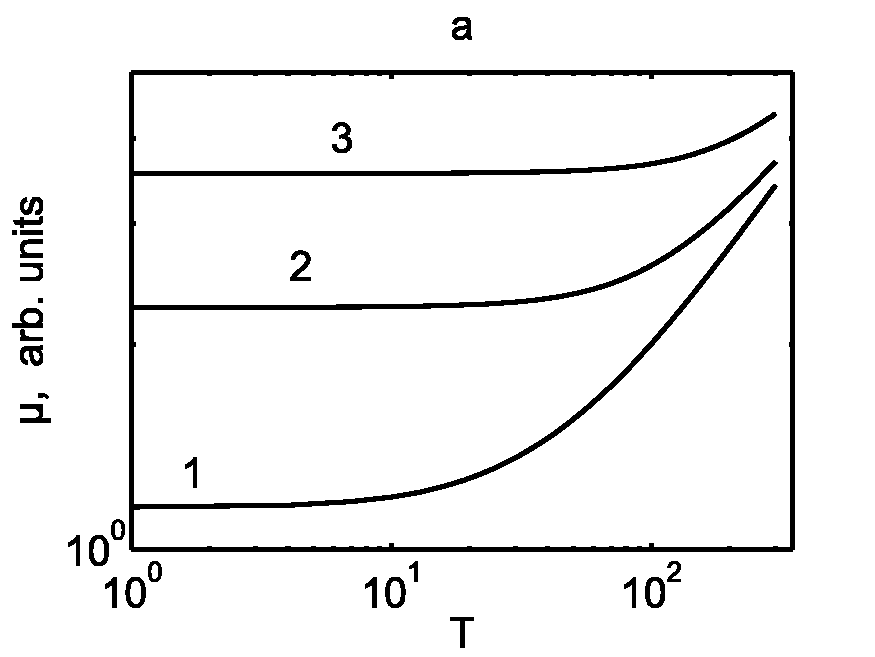
\includegraphics [scale=1] {fig_3_1_1}
	\caption{Температурная зависимость подвижности (в относительных единицах) при учете рассеяния носителей на шероховатой поверхности в КЯ при $\Lambda =70 \AA$, $\Delta =3 \AA$, $L_{0} = 100 \AA$, кривые 1, 2, 3 получены соответственно для $n_{s} = 10^{11} \text{cm}^{-2}$, $n_{s} = 7 \cdot 10^{11} \text{cm}^{-2}$,$n_{s} = 1.5 \cdot 10^{12} \text{cm}^{-2}$.}
	\label{img:fig_3_1_1} 
\end{figure}

Следовательно, подвижность существенным образом зависит от толщины размерно-квантованной системы $(\mu_0 \sim L^6 )$. На рисунке~\ref{img:fig_3_1_1} (кривая 1) приведена температурная зависимость $\mu ^{(nd)} /\mu_0 $ с учетом зависимости химического потенциала от температуры \eqref{eq:31_190}. Как непосредственно следует из рисунка~\ref{img:fig_3_1_1}, при низких $T$ $(\delta \gg 1)$ подвижность практически не зависит от температуры и при высоких температурах $(\delta <1)$ с ростом $T$ увеличивается (кривая 1). Такое поведение подвижности от $L$ и $T$ экспериментально наблюдалось в GaAs/AlAs \cite{Sakaki1987}. При низких температурах $\mu ^{(nd)} =\mu_0 $, т.е. определяется только размером КЯ и параметрами флуктуирующей поверхности $\Delta $, $\Lambda $. При изменении толщины КЯ от $70 \AA$ до $100 \AA$ подвижность изменяется от $\mu_0 =2.6\cdot 10^3 \text{cm}^2 / \text{Vs}$ до $\mu_0 =2\cdot 10^4 \text{cm}^2 /\text{Vs}$, что согласуется с экспериментальными данными в КЯ GaAs/AlAs \cite{Sakaki1987}.

Для вырожденного электронного газа при низких $T$ электропроводность принимает вид:
\begin{equation} \label{eq:31_210}
\sigma _{xx}^{(d)} =\frac{e^2 \hbar \tilde{\xi }}{\pi^2 L m_e \left(\Delta \Lambda V_{1} \right)^2 } \frac{\exp{\left(\frac{m_e \Lambda^2 }{\hbar^2 } \tilde{\xi }\right)}}{\mathrm{I}_0 \left(\frac{m_e \Lambda^2 }{\hbar^2 } \tilde{\xi }\right)}.
\end{equation}
Если $\beta_0 \pi \hbar^2 n_s /m_e \gg 1$, то $\tilde{\xi }=\pi \hbar^2 n_s /m_e$ и подвижность определяется соотношением:
\begin{equation} \label{eq:31_220}
\mu^{(d)} =\mu _{0} \frac{\exp (a)}{\mathrm{I}_0 (a)},
\end{equation}
\[
a=\pi \Lambda ^{2} n_{s}
\]
При $a \ll 1 \; (\mathrm{I}_0 (a) \simeq 1)$ 
\begin{equation} \label{eq:31_230}     
\mu ^{(d)} =\mu _{0}.
\end{equation}
При $a \gg 1  \; (\mathrm{I}_0 (a) \simeq e^a / \sqrt{2\pi a})$
\begin{equation} \label{eq:31_240}  
\mu ^{(d)} =\mu _{0} \pi \sqrt{2\Lambda ^{2} n_{s} }
\end{equation}

Как следует из \eqref{eq:31_230} в исследуемой модели КЯ подвижность в области низких температур не зависит от $T$ (кривая 2 на рисунке~\ref{img:fig_3_1_1}). Такое поведение $\mu^{(d)} $ от $T$ экспериментально наблюдалось в кремниевых инверсионных слоях, в которых электронный газ остается вырожденным вплоть до $T<100 K$ ($\tilde{\xi }=12.5 \text{meV}$, $n_{s} =2\cdot 10^{12} \text{cm}^{-2} $) \cite{Stern1980}. Для $\Delta =6\AA$, $\Lambda =13 \AA$, при $L=70 \AA$, $n_{s} =2\cdot 10^{12}  \text{cm}^{-2} $ $(a \ll 1)$ $\mu^d =1.5 \cdot 10^4 \text{cm}^2 /\text{Vs}$, что близко к экспериментальным данным \cite{Stern1980}.

Аналогичные расчеты подвижности можно провести для прямоугольной квантовой ямы при $\delta$-образной флуктуации поверхности. Учитывая предельный переход от гауссовой флуктуации поверхности к $\delta $-образной, когда $\Lambda \to 0$, ${\left(\Delta \Lambda \right)}^2\to \pi \gamma $ (см. замечание в \ref{sect1_2}) можно получить выражение для электропроводности. Согласно \eqref{eq:31_180} электропроводность в этом случае может быть записана в виде:

\begin{equation} \label{eq:31_250}
{\sigma }^{\delta }_{xx}=\frac{e^2\hbar }{{\pi }^3{\beta }_0 m_e L V^2_0 \gamma_0 }\int\limits_0^\infty{\frac{x dx \exp{(x-\beta \widetilde{\xi })}}{{\left[ \exp{(x-\beta \widetilde{\xi })}+1 \right] }^2}}
\end{equation}
Из \eqref{eq:31_250} не трудно получить выражения для подвижности вырожденного и невырожденного электронного газа: 
\begin{equation} \label{eq:31_260}
\mu^{\delta \left(d\right)} = \mu^{\delta \left(n d\right)}=\frac{e L^6}{\hbar {\pi }^6\gamma },
\end{equation}
которые совпадают и существенным образом зависит от размеров квантовой системы и не зависят от температуры

Для КП потенциал взаимодействия носителей с шероховатой поверхностью определяется \eqref{eq:1_1} и в случае гауссовской флуктуации поверхности автокорреляционная функция для различных точек поверхности записывается в виде \eqref{eq:1_6}. С учетом волновых функций для квантовой проволоки \cite{Constantinou1989} $W_{\gamma \alpha } $ легко вычисляется и $\tau_{\alpha }^{-1} $ принимает следующий вид:
\begin{equation} \label{eq:31_290}
\frac{1}{\tau _{\alpha } } =\frac{(\Delta \tilde{V}_0 )^2 m\Lambda \sqrt{\pi } }{\hbar^3 \left|k_x \right|} \left\{1+ \exp\left[-\left(k_x \Lambda \right)^2 \right]\right\}.
\end{equation}
Подставляя \eqref{eq:31_290} в \eqref{eq:31_150} и интегрируя по квазиимпульсу электрона $\hbar k_x $ нетрудно получить:
\begin{equation} \label{eq:31_300}
\sigma_{xx} =\frac{2 e^2 \hbar^3 \delta }{m^2 \pi^2 \sqrt{\pi } R_0^2 (\Delta \Lambda \tilde{V}_1 )^2 \Lambda } \cdot \int \limits_0^{\infty }{d\tau \frac{\tau \cdot \exp(\delta \tau -\beta_0 \tilde{\xi })}{\left[ \exp(-\tau )+1\right] \cdot \left[ \exp(\delta \tau -\beta_0 \tilde{\xi })+1\right]^2 }},
\end{equation}
$\beta_0 \tilde{\xi }$ определяется из уравнения:
\[
\sum_{\alpha } {f_{\alpha}(\tilde{\xi }) = N},
\]
которое приводится к виду:
\begin{equation} \label{eq:31_305}
\int\limits_0^{\infty }{\frac{dx}{\exp \left(x^{2} -\beta _{0} \tilde{\xi }\right)+1}} =\frac{n_{l} \pi \hbar \sqrt{\beta _{0} } }{\sqrt{8m} },
\end{equation}
$n_{l} =N/L_{x} $ -- линейная плотность электронов.

\begin{figure}[h]  
	\center
	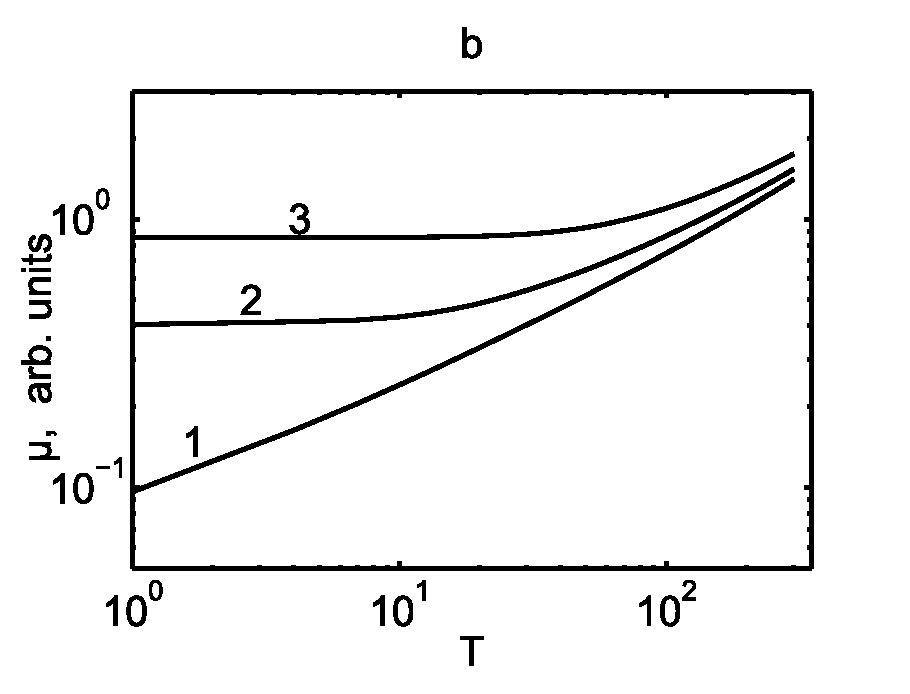
\includegraphics [scale=1] {fig_3_1_2}
	\caption{Температурная зависимость подвижности (в относительных единицах) при учете рассеяния носителей на шероховатой поверхности в КП при $\Lambda =20 \AA$, $\Delta =2 \AA$, $R_{0}=100 \AA$, кривые 1, 2, 3 получены соответственно для $n_{l} = 10^5 \text{cm}^{-1}$, $n_l = 5 \cdot 10^5 \text{cm}^{-1}$,$n_{s} = 10^6 \text{cm}^{-1}$.}
	\label{img:fig_3_1_2}	
\end{figure}

На рисунке~\ref{img:fig_3_1_2} представлена температурная зависимость электропроводности (в относительных единицах) в КП с учетом зависимости химического потенциала от концентрации носителей и температуры \eqref{eq:31_305}. Для невырожденного электронного газа (кривая 1 на рисунке~\ref{img:fig_3_1_2}) электропроводность имеет корневую зависимость от температуры ($\sigma_{xx}^{(nd)} \sim \sqrt{T} $).

Для вырожденного электронного газа искомая электропроводность (рассматривается нижайшая электронная зона) записывается в следующем виде:
\begin{equation} \label{eq:31_310}
\sigma _{xx}^{(d)} =\frac{4 e^2 \hbar \tilde{\xi }}{\pi^2 \sqrt{\pi } R_0^2 m \left(\Delta \tilde{V}_1 \right)^2 \Lambda } \cdot \frac{1}{1+{\exp}(-q)} , q=\frac{2m\Lambda^2 }{\hbar^2 } \tilde{\xi }.  
\end{equation}

Как непосредственно следует из \eqref{eq:31_310}, для вырожденных КП электропроводность, а следовательно и подвижность, при низких температурах не зависит от T (кривая 3 на рисунке~\ref{img:fig_3_1_2}). Такое поведение электропроводности от температуры экспериментально наблюдалось в КП Bi \cite{Lin2000,Heremans1998,Zhang2000,Heremans2000,Gitsu2003,Nikolaeva2006,Gitsu2005}.

Из рисунках~\ref{img:fig_3_1_1}-\ref{img:fig_3_1_2} следует, что электропроводность при рассеянии носителей на шероховатой поверхности размерно-квантованной системы в области низких температур слабо (для невырожденных квантовых систем) или вообще не зависит (для вырожденного электронного газа) от T. При этом с ростом T $\sigma _{xx} $, а следовательно и подвижность, начинает увеличиваться. Однако как показывают экспериментальные исследования \cite{Zhang2000,Gitsu2003,Nikolaeva2006} при высоких температурах подвижность уменьшается. Следовательно «включается» другой механизм рассеяния носителей, например, на колебаниях решетки. Поэтому для последовательного сравнения теории с экспериментом рассмотрим температурную зависимость электропроводности с учетом двух механизмов рассеяния (на неровностях поверхности и на фононах). Это обстоятельство позволяет исследовать поведение подвижности в широкой области температур ($T\le 200\text{K}$).

В приближении времени релаксации, если использовать соотношение \eqref{eq:31_120} и результаты работы \cite{Khamidullin2002} выражение для электропроводности записывается следующим образом

\begin{equation} \label{eq:31_320}
\sigma _{xx} =\frac{\beta_0 e^2 }{Vm^2 } \sum _{\alpha }\left|\hat{p}_{\alpha \alpha }^{(x)} \right|^{2} \frac{\tau _{\alpha } \tau_{\alpha }^f }{\tau_{\alpha } +\tau_{\alpha }^f } n_{\alpha } \left(1-n_{\alpha } \right),
\end{equation}
$\tau _{\alpha } $ --- время релаксации, определяемое рассеянием электронов на шероховатой поверхности, $\tau_{\alpha }^f $ --- время релаксации, связанное с рассеянием электрона на фононах \cite{Khamidullin2002}.

Для прямоугольной КЯ при рассеянии электронов в нижайшей зоне проводимости:
\begin{equation} \label{eq:31_330}
\frac{1}{\tau_{\alpha }^f } = \frac{3 E_1^2 m}{\beta_0 \hbar^3 \rho \nu^2 L},
\end{equation}
здесь $E_1 $ -- константа деформационного потенциала для электрона, $\nu $ -- скорость звука в кристалле с плотностью $\rho $.

Для КП с бесконечным потенциалом для нижайшей зоны проводимости:
\begin{equation} \label{eq:31_340}
\frac{1}{\tau _{\alpha }^f } =\gamma_f \frac{1}{\left|k_{x} \right|}, \;
\gamma_f =\frac{4 E_1^2 m}{\beta_0 \hbar^3 \rho \nu^2 \pi R_0^2 },
\end{equation}
выражение для электропроводности прямоугольной КЯ записывается в виде:
\begin{multline} \label{eq:31_350}
\sigma _{xx} =\frac{e^2 \hbar^3 }{\pi^2 m^2 \left(\Delta \Lambda^2 V_1 \right)^2 L} \delta^2 \gamma \times \\
 \times \int\limits_0^{\infty }{d\tau \frac{\tau \cdot \exp (\delta \tau -\beta \tilde{\xi })}{\left[\delta \gamma \cdot \exp(-\tau ) \mathrm{I}_0 (\tau )+1\right]\cdot \left[\exp(\delta \tau -\beta \tilde{\xi })+1\right]^{2} }},
\end{multline}
\[
\delta =\frac{\hbar^2 \beta_0 }{m \Lambda^2 }, \;
\gamma =\frac{\pi m\rho \nu^2 L}{3\hbar^2 E_1^2 } \left(\Delta \Lambda^2 V_1 \right)^2 .
\]
 
Для невырожденного электронного газа подвижность определяется соотношением:
\begin{equation} \label{eq:31_360}
\mu ^{(nd)} =\mu_0 \cdot \delta^3 \gamma \int\limits_0^{\infty}{d\tau \frac{\tau \cdot \exp(-\tau \delta )}{\delta \gamma \cdot \exp(-\tau ) \mathrm{I}_0 (\tau )+1}}. 
\end{equation}

Если $\delta \gamma \ll 1$, то из \eqref{eq:31_360} получается выражение для подвижности, связанное с рассеянием носителей на длинноволновых колебаниях:

\begin{equation} \label{eq:31_370}
\mu _{xx}^{(fnd)} =\frac{e\hbar ^{3} \rho \nu ^{2} L^{2} }{3m^{2} E_{1}^{2} } \beta _{0}. 
\end{equation}

Для типичных параметров КЯ GaAs/AlAs ($\rho =5.4 \text{ g} / \text{cm}^3 $, $v=5\cdot 10^5 \text{ cm/s}$, $E_1 =7 \text{ eV}$, $m=0.06m_{0} $) при $\Delta =3 \AA$, $\Lambda =70 \AA$, $L = 100 \AA$  $\gamma \delta \cong 520/\text{T}$ и, следовательно, при $T>100\text{ K}$ рассеяние носителей на фононах начинает заметно влиять на температурную зависимость подвижности.

Для случая вырожденного электронного газа:
\begin{equation} \label{eq:31_380}
\sigma _{xx}^{(d)} =\frac{e^2 \hbar^3 }{\pi^2 m^2 \left(\Delta \Lambda^2 V_0 \right)^2 L} \cdot 
\frac{\delta \gamma \cdot \delta_0 }{\delta \gamma \cdot \mathrm{I}_0 \left(\delta_0 \right)\exp\left(-\delta_0 \right)+1} ,
\end{equation}
$n_s $ -- поверхностная плотность электронов, $\delta_0 =\pi \Lambda^2 n_s $.

При $\delta \gamma \gg 1$ из \eqref{eq:31_380} получается выражение для подвижности \eqref{eq:31_220}. Если $\delta \gamma \ll 1$, то из \eqref{eq:31_380} следует соотношение для подвижности в прямоугольной квантовой яме, когда учитывается взаимодействие носителей с длинноволновыми фононами:
\begin{equation} \label{eq:31_390}
\mu _{xx}^{(fd)} =\frac{e\hbar^3 \rho \nu^2 L\beta_0 }{3 m^2 E_1^2 }. 
\end{equation}
 
Аналогичным образом можно вычислить электропроводность для квантовых проволок с бесконечным потенциалом, используя соотношения \eqref{eq:31_300}, \eqref{eq:31_340}:
\begin{multline} \label{eq:31_400}
\sigma _{xx} =\frac{2e^2 \hbar^3 \delta^2 q}{m^2 \pi^2 \sqrt{\pi } R_0^2 \left(\Delta \Lambda V_1 \right)^2 \Lambda } \times\\
\times\int\limits_0^{\infty} {d\tau \frac{\tau \cdot {\exp}\left(\delta \tau -\beta _{0} \tilde{\xi }\right)}{\left[\delta q\cdot \left(\exp(-\tau) +1 \right)+1\right]\cdot \left[{\exp}\left(\delta \tau -\beta _{0} \tilde{\xi }\right)+1\right]^{2} }}, 
\end{multline}
\[
\delta =\frac{\beta_0 \hbar^2 }{2m\Lambda^2 }, \;
q=\frac{m \rho \nu^2 \sqrt{\pi } \pi R_0^2 }{2\hbar^2 E_1^2 } \left(\Delta \Lambda V_0 \right)^2 \Lambda .
\] 

Для невырожденного электронного газа квантовой проволоки \eqref{eq:31_400} принимает вид:
\begin{equation} \label{eq:31_410}
\sigma_{xx}^{(nd)} =\frac{2e^2 \hbar^3 n_e }{\pi m_e^2 \left(\Delta \Lambda V_0 \right)^2 } q \delta ^{\frac{5}{2} }
\int\limits_0^{\infty }{d\tau \frac{\tau \cdot \exp (-\delta \tau )}{\left[\delta q\cdot \left( \exp(-\tau )+1\right)+1\right]}}. 
\end{equation}

При $\delta q \ll 1$ из \eqref{eq:31_410} непосредственно следует выражение для электропроводности, связанное с рассеянием электронов на длинноволновых (акустических) фононах:
\begin{equation} \label{eq:31_420}
\sigma _{xx}^{(nd)} =\frac{e^2 \hbar^2 n_e R_0^2 \rho \nu^2 }{m E_1^2 } \sqrt{\frac{\beta_0 \pi }{2m_e} }
\end{equation}

Для вырожденного электронного газа:
\begin{equation} \label{eq:31_430}
\sigma _{xx}^{(d)} =\frac{2 e^2 \hbar^3 }{\pi^2 R_0^2 m_e^2 \sqrt{\pi } \left(\Delta \Lambda V_0 \right)^2 \Lambda } \cdot \frac{\delta q \cdot \delta_1 }{\delta q\cdot \left(1+{\exp}(-\delta_1 )\right)+1}, 
\end{equation}
\[
\delta_1 =\frac{2 m_e\Lambda^2 }{\hbar^2 } \tilde{\xi }. 
\]
Если $\delta q\gneq1$, то электропроводность имеет вид:
\begin{equation} \label{eq:31_440}
\sigma _{xx}^{(fnd)} =\frac{e^2 \hbar \rho \nu^2 \beta_0 }{\pi m E_1^2 } \tilde{\xi }.
\end{equation}

\begin{figure}[h]  
	\center
	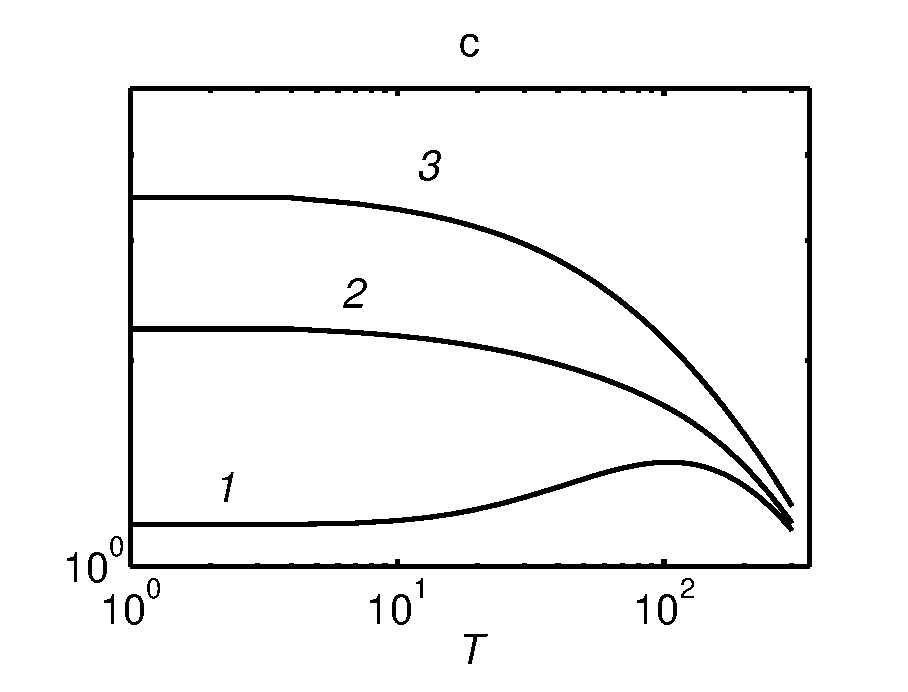
\includegraphics [scale=1] {fig_3_1_3}
	\caption{Температурная зависимость подвижности (в относительных единицах) при учете рассеяния носителей на шероховатой поверхности и на фононах в КЯ при $\Lambda =70 \AA$, $\Delta =3 \AA$, $L_{0}=100 \AA$, кривые 1, 2, 3 получены соответственно для $n_s = 10^{11} \text{cm}^{-2}$, $n_s = 7 \cdot 10^{11} \text{cm}^{-2}$, $n_s = 1.5 \cdot 10^{12} \text{cm}^{-2}$.} 
	\label{img:fig_3_1_3}	
\end{figure}

На рисунке~\ref{img:fig_3_1_3} приведена температурная зависимость подвижности (в относительных единицах) для различных концентраций носителей в прямоугольной КЯ. Для невырожденного электронного газа (кривая 1) подвижность немонотонным образом зависит от T, что экспериментально наблюдалось в КЯ GaAs/AlAs \cite{Sakaki1987}. Заметим, что с ростом ширины КЯ уменьшается влияние рассеяния носителей на шероховатости поверхности, поэтому максимум подвижности смещается в область низких температур. Кривые 2, 3 описывают температурную зависимость подвижности для вырожденного электронного газа. При низких T подвижность практически не зависит от температуры и с ее ростом уменьшается. Именно такое поведение подвижности от температуры экспериментально наблюдалось в инверсионных слоях Si для вырожденного электронного газа \cite{Stern1980}.

\section{ Электропроводность в размерно-квантовых системах с учётом рассеяния носителей на шероховатой поверхности в магнитном поле}

Рассмотрим особенности электропроводности, возникающие в размерно-квантованных системах в присутствии однородного магнитного поля напряжённостью $\vect{H}$. Для параболических КЯ в продольном магнитном поле ($\vect{H} || OX$) электропроводность для основного состояния описывается соотношением:
\begin{equation} \label{eq:32_10}
\sigma_{xx} =\frac{e^2 \hbar^3 n}{m^2 \gamma V_0^2 } \left[\frac{\omega }{\Omega } \right],
 \end{equation}
 \begin{equation} \label{eq:32_20}
 V_0 =\frac{\hbar }{2} \left(\frac{\omega }{\Omega } \right)\frac{\partial \omega }{\partial L} .
 \end{equation}
\[
\Omega^2 =\omega^2 +\omega_c^2,
\] 
\[
\hbar \omega =\frac{1}{L} \left(\frac{8\Delta E_c }{m} \right)^{\frac{1}{2} } 
\]
-- шаг пространственного квантования, $\omega _{c} $-- циклотронная частота, $n$-- концентрация носителей.

С учётом \eqref{eq:32_10}, \eqref{eq:32_20} подвижность для электронного газа с произвольным вырождением принимает вид:

\begin{equation} \label{eq:32_30}
\mu _{xx} =\frac{4e\hbar }{m^{2} \gamma } \left(\frac{\partial \omega }{\partial L} \right)^{-2} \left[1+\left(\frac{\omega _{c} }{\omega } \right)^{2} \right]^{\frac{1}{2} }.
\end{equation}

Заметим, что подвижность в размерно-ограниченных системах при учёте рассеяния носителей на длинноволновых колебаниях с ростом магнитного поля уменьшается \cite{Sinyavskii1998}. Это связано с ростом локализации зонных электронов. Как непосредственно следует из \eqref{eq:32_30} $\mu _{xx} $ с ростом магнитного поля увеличивается. Такое поведение зависимости подвижности от продольного магнитного поля может быть понято из следующих соображений. В параболической КЯ радиус локализации электрона $\lambda _{0} =\sqrt{\frac{\hbar }{m\Omega } } $ с ростом напряженности магнитного поля уменьшается, число носителей тока, рассеивающихся на шероховатой поверхности размерно-ограниченной системы, становится меньше, что и приводит к росту подвижности.

В поперечном магнитном поле в плоскости КЯ ($\vect{H} || OY$) матричные элементы обобщённого импульса, входящие в общее выражение для электропроводности \eqref{eq:31_150} определяются следующим образом:
\begin{equation} \label{eq:32_40}
P_{\alpha \beta }^{\left(x\right)} =\hbar k_{x} \left(\frac{\omega }{\Omega } \right)\delta _{\alpha \beta } -\frac{m\omega _{c} }{\sqrt{2} \lambda } \delta _{k_{x} k'_{x} } \delta _{k_{y} k'_{y} } \left\{\sqrt{n} \delta _{n,n_{1} +1} +\sqrt{n+1} \delta _{n,n_{1} +1} \right\}.
\end{equation}
Следовательно, матричный элемент обобщенного импульса имеет как диагональные элементы (первое слагаемое в \eqref{eq:32_40}), так и недиагональные элементы по квантовому числу размерно-магнитного квантования (второе слагаемое). Заметим, что диагональный матричный элемент возникает только в размерно-ограниченных системах (при $\omega \to 0$ это слагаемое в \eqref{eq:32_40} отсутствует).

В дальнейшем будем рассматривать электропроводность с учётом диагонального слагаемого в матричном элементе обобщенного импульса. Подвижность в поперечном магнитном поле при низких температурах для основного состояния имеет вид:
\begin{equation} \label{eq:32_50}
\mu _{x} =\frac{4e\hbar }{m^{2} \gamma } \left(\frac{\partial \omega }{\partial L} \right)^{-2} \left[1+\left(\frac{\omega _{c} }{\omega } \right)^{2} \right]^{-\frac{1}{2} }
\end{equation}
Следовательно, с ростом магнитного поля подвижность уменьшается и при $\left(\frac{\omega _{c} }{\omega } \right)^{2} \gg 	1$ $\mu _{x} \sim \frac{1}{H} $. Такое поведение подвижности от $H$связано с тем, что в скрещенных магнитном и электрическом полях носители с дрейфовой скоростью перемещаются вдоль оси пространственного квантования по трохоиде, поэтому активно участвуют в процессах рассеяния на шероховатостях поверхности размерно-квантовой системы. 

Рассмотрим электропроводность в квантовых проволоках в однородном магнитном поле. В продольном магнитном поле время релаксации, определяемое \eqref{eq:31_140}, вычисляется обычным образом. В результате
\begin{equation} \label{eq:32_60}
\frac{1}{\tau _{\alpha } } =\frac{\gamma _{0} }{\hbar ^{3} } 2mV_{\alpha }^{2} \frac{1}{\left|k_{x} \right|} . 
\end{equation}

Электропроводность \eqref{eq:31_150} в рассматриваемой модели параболической КП принимает вид:
\begin{equation} \label{eq:32_70}
\sigma _{xx} =\frac{4\hbar e^{2} }{2\beta \pi sm\gamma _{0} } \sum _{n\nu }\frac{1}{V_{n\nu }^{2} } \ln \left[1+\exp \left\{\beta \xi _{n\nu } \right\}\right]
\end{equation}
\[
V_{\alpha } =\frac{4}{\left[4+\delta ^{2} \right]^{\frac{1}{2} } } \left[n+\frac{1}{2} +\frac{\left|\nu \right|}{2} \right]\frac{\partial (\hbar \omega )}{\partial R_{0} } .
\] 
При этом $\xi _{n\nu } $определяется из уравнения для химического потенциала параболической КП:
\begin{equation} \label{eq:32_80}
\sum _{n\nu }\int _{0}^{\infty }\frac{dx}{1+e^{x^{2} -\beta \xi _{n\nu } } } =\frac{\pi n_{e} }{2} \left(\frac{\hbar ^{2} \beta }{2m} \right)^{\frac{1}{2} } 
\end{equation}

Для невырожденного электронного газа из \eqref{eq:32_80} следует:
\[
\sum _{n\nu }e^{\beta \xi _{n\nu } }  =n_{e} \left[\frac{\pi \hbar ^{2} \beta }{2m} \right]^{\frac{1}{2} } .
\] 
И, следовательно, для основного размерно-квантового состояния ($n=\nu =0$) подвижность записывается в виде:
\begin{equation} \label{eq:32_90}
\mu _{x}^{\left(nd\right)} =\frac{eR_{0}^{4} \left[4+\left(\frac{\omega _{c} }{\omega } \right)^{2} \right]}{4\gamma _{0} \left(\Delta E_{c} \right)\sqrt{2m\beta \pi } } . 
\end{equation}
В случае вырожденного электронного газа из \eqref{eq:32_80} нетрудно получить
\[
\sum _{n\nu }\sqrt{\xi _{n\nu } }  =\pi n_{e} \left[\frac{\hbar ^{2} }{2m} \right]^{\frac{1}{2} } .
\] 
и для основного электронного состояния ($n=\nu =0$) подвижность определяется соотношением:
\begin{equation} \label{eq:32_100}
\mu _{x}^{\left(d\right)} =\frac{e\pi \left[4+\left(\frac{\omega _{c} }{\omega } \right)^{2} \right]n_{e} \hbar R_{0}^{4} }{8m\gamma _{0} \left(\Delta E_{c} \right)} .
\end{equation}
 
Следовательно, в продольном магнитном поле, подвижность, увеличивается ($\mu _{x} \sim H^{2} $ ) и существенным образом зависит от радиуса квантовой проволоки ($\mu _{x} \sim R_{0}^{4} $). Если для невырожденного электронного газа  подвижность \eqref{eq:32_90} увеличивается с ростом температуры, то для вырожденной размерно-квантовой проволоки подвижность при низких температурах не зависит от $T$. На рис. \ref{img:fig_3_2_1} представлена зависимость сопротивления (в относительных единицах) от напряженности магнитного поля с учетом рассеяния носителей на шероховатой поверхности (пунктирная линия). Сплошной линией представлена зависимость относительного сопротивления от магнитного поля для нанопроволок висмута с учетом рассеяния на шероховатой поверхности и при упругом рассеянии на акустических фононах. Именно, такая зависимость сопротивления от магнитного поля экспериментально наблюдалась в работе \cite{Nikolaeva2004}.

\begin{figure}[h] 
	\center
	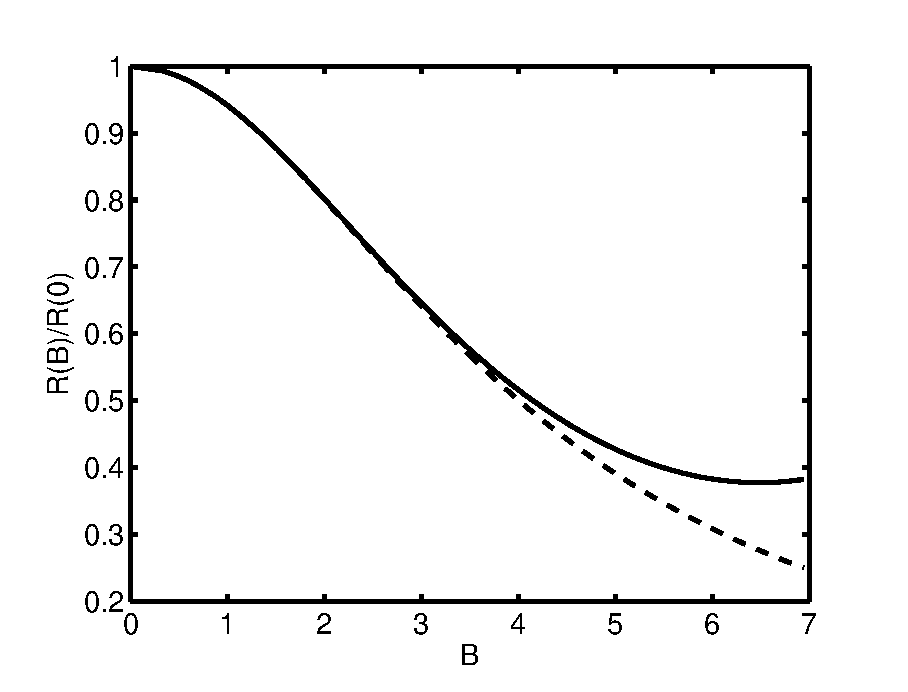
\includegraphics [scale=1] {fig_3_2_1}
	\caption{Зависимость относительного сопротивления от магнитного поля для нанопроволоки висмута ($d=80 \text{ nm}$, $T=4.2\text{ K}$). Пунктирной линией показана зависимость $R(H)/R(0)$ при учете рассеяния носителей на поверхности, сплошной линией при учете рассеяния носителей на шероховатой поверхности и на акустических фононах.} 
	\label{img:fig_3_2_1} 
\end{figure}